\documentclass[../informe_krapp.tex]{subfiles}
\begin{document}
\section{Partes del proyecto}
\subsection{El protocolo de comunicación SPI}
\begin{wrapfigure}{r}{0in}
	\centering
	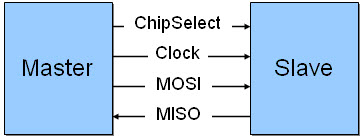
\includegraphics[width= 1.5in, keepaspectratio]{spi-1.jpg}
\end{wrapfigure}

El protocolo Serial Peripheral Interface es un protocolo de comunicación creado por
Motorola, anunciado en el año 1979.
El mismo se divide en 4 lineas de comunicación, cada una con una función específica
(por favor, ver figura \ref{spi-single-slave}) con:

\begin{itemize}
	\item Una señal de clock llamada SCLK, enviada desde el bus master a todos los slaves.
	      Todas las señales del protocolo van as er sínconas a esta señal de clock
	\item Una señal de selección de slave llamada SSn, usada para seleccionar con
	      que slave se esta comunicando el master
	\item Una linea de datos desde master hacia slave, llamada MOSI (Master Out Slave In)
	\item Una linea de datos desde slave hacia master, llamada MISO (Master In Slave OUT)
\end{itemize}

\begin{figure}[H]
	\centering
	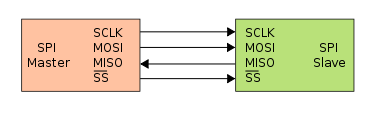
\includegraphics[width=0.5\textwidth]{spi-single-slave.png}
	\caption{SPI master conectado a un único slave.}
	\label{spi-single-slave}
\end{figure}

\begin{figure}[H]
	\centering
	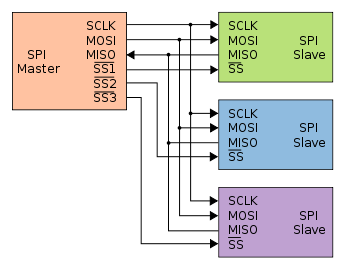
\includegraphics[width=0.5\textwidth]{spi-multiple-slaves.png}
	\caption{SPI master conectado a múltiples slaves.}
	\label{spi-multiple-slaves}
\end{figure}

\todo{no olvidarse de la daisy chained}

\clearpage

SPI es un protoclo de comunicación single-master, esto significa que un dispositivo
central (normalmente un microcontrolador) es el encargado de iniciar todas
las comunicaciónes con los slaves.

Cuando el master SPI desea enviar o recibir información de un slave, selecciona el
slave seteando en LOW la linea SS correspondiente, y activa la señal de clock a una
frecuencia usable por el master y el slave.
A partir de ese momento, el master envía la información por el canal MOSI mientras lee
la información que hay en el canal MISO

\begin{figure}[H]
	\centering
	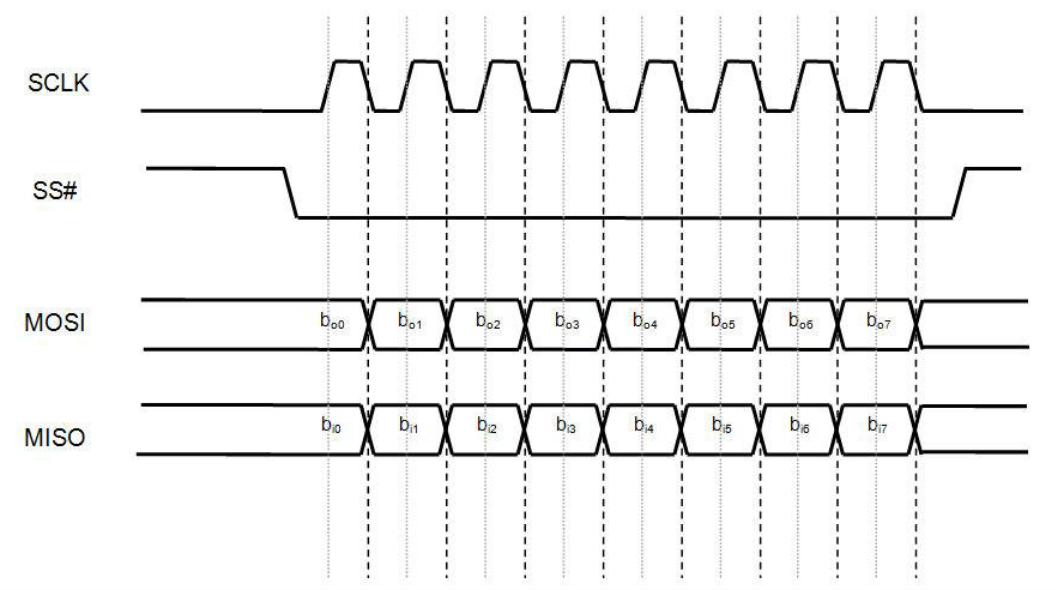
\includegraphics[width=0.7\textwidth]{spi-timing.png}
	\caption{El timing de una comunicación SPI. En este ejemplo,
		La transmisión de datos por los canales MOSI y MISO es ejecutada por
		cada flanco descendente en la señal de clock en SCLK. En cambio,
		la lectura de datos es ejecutada por cada flanco ascendente.
		Esto se puede cambiar modificando el SPI mode }
	\label{spi-timing}
\end{figure}

Como se menciona en la figura \ref{spi-timing}, hay 4 modos SPI, que van del 0 al 3.
Los modos SPI definen en que flanco se activa la linea MOSI, MISO, y el estado (LOW o HIGH)
de inactividad (idle) del canal SCLK.
Cada modo esta definido por un par de parámetros llamados clock polarity
(polaridad de clock) (CPOL), y clock phase (fase de clock) (CPHA)

\begin{figure}[H]
	\centering
	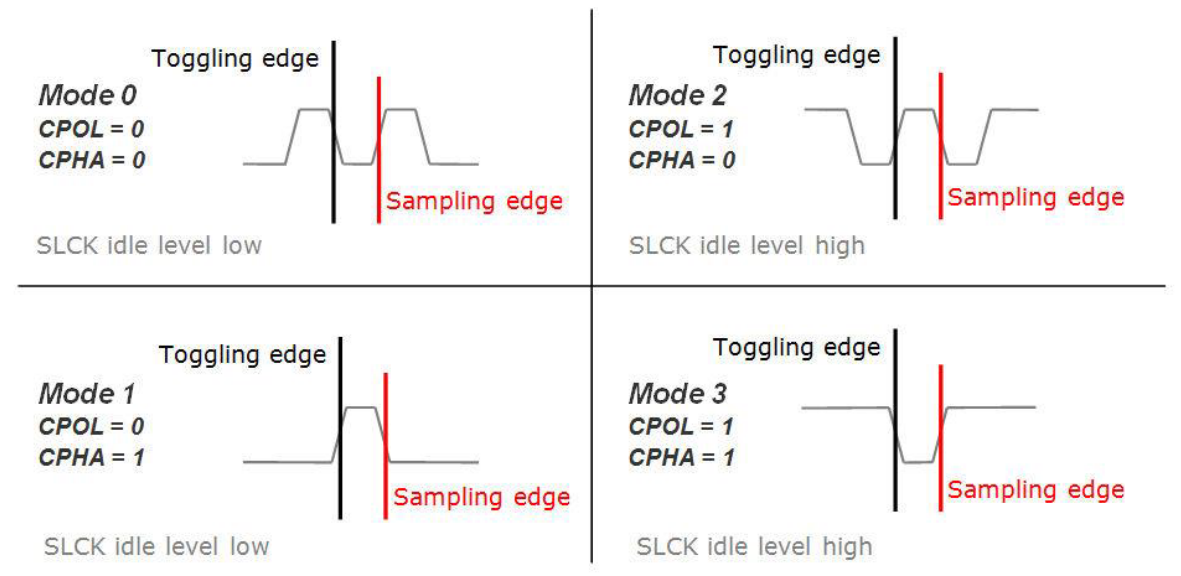
\includegraphics[width=0.7\textwidth]{spi-modes.png}
	\caption{Los modos SPI son definidos con los parámetros CPOL (clock polarity) y CPHA
		(clock phase), que definen 3 parámetros: El flanco usado para envío de datos, el
		flanco usado para recepción de datos, y el estado de inactividad (idle) de SCLK}
	\label{spi-modes}
\end{figure}

Una conexión SPI master/slave tiene que usar el mismo set de parámetros explicados
en la figura \ref{spi-modes} para poder efectuar una comunicación.
Si de todas formas se desea que múltiples slaves tengan configuraciones distintas,
el master deberá reconfigurarse cada vez que se desee comunicar con cada dispositivo.
\begin{figure}[H]
	\centering
	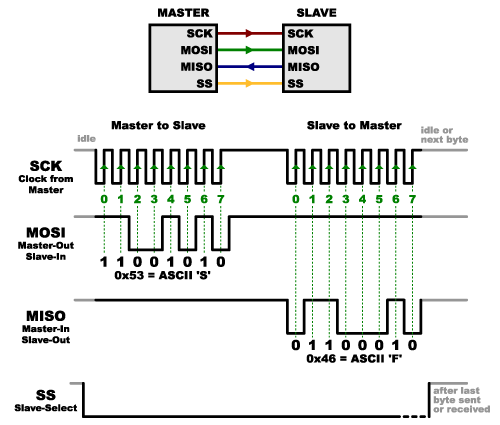
\includegraphics[width=0.7\textwidth]{spi-timing-2.png}
	\caption{Grafico de comunicacion SPI}
\end{figure}

\subsubsection{Ventajas y desventajas}

\todo{ventajas y desventajas}









\clearpage

\subsection{DOIT ESP32 DevKit v1}
\begin{wrapfigure}{r}{0in}
	\centering
	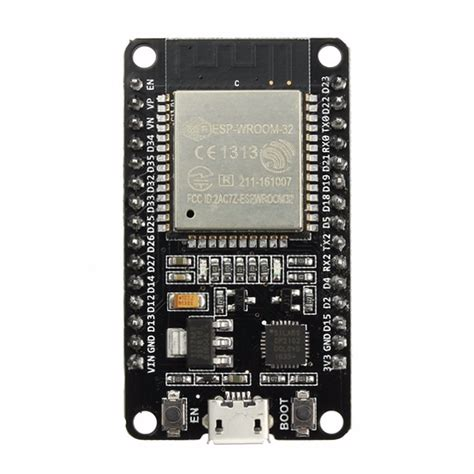
\includegraphics[width= 1.5in, keepaspectratio]{ESP32-board.jpg}
\end{wrapfigure}
El kit de desarrollo DOIT ESP32 DevKit v1



\clearpage
\subsection{RFID}
Segun Wikipedia\cite{wikipedia_rfid_es}:

\begin{center}
	\rule{0.9\textwidth}{0.5pt}
\end{center}
``RFID o identificación por radiofrecuencia
(del inglés Radio Frequency Identification) es un sistema de almacenamiento y recuperación
de datos remotos que usa dispositivos denominados etiquetas, tarjetas o transpondedores
RFID.

\begin{wrapfigure}{r}{0in}
	\centering
	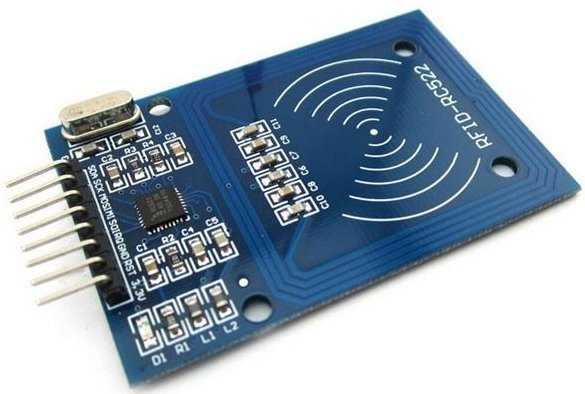
\includegraphics[width= 1.5in, keepaspectratio]{rfid-rc552.jpg}
\end{wrapfigure}

El propósito fundamental de la tecnología RFID es transmitir la identidad de
un objeto (similar a un número de serie único) mediante ondas de radio. Las tecnologías
RFID se agrupan dentro de las denominadas Auto ID (automatic identification,
o identificación automática).

Las etiquetas RFID (RFID tag en inglés) son unos dispositivos pequeños, similares
a una pegatina, que pueden ser adheridas o incorporadas a un producto, un animal
o una persona. Contienen antenas para permitirles recibir y responder a peticiones
por radiofrecuencia desde un emisor-receptor RFID. Las etiquetas pasivas no necesitan
alimentación eléctrica interna, mientras que las activas sí lo requieren.

Una de las ventajas del uso de radiofrecuencia (en lugar, por ejemplo, de infrarrojos)
es que no se requiere visión directa entre emisor y receptor''

\begin{center}
	\rule{0.9\textwidth}{0.5pt}
\end{center}

\begin{figure}[H]
	\centering
	\begin{subfigure}{0.4\textwidth}
		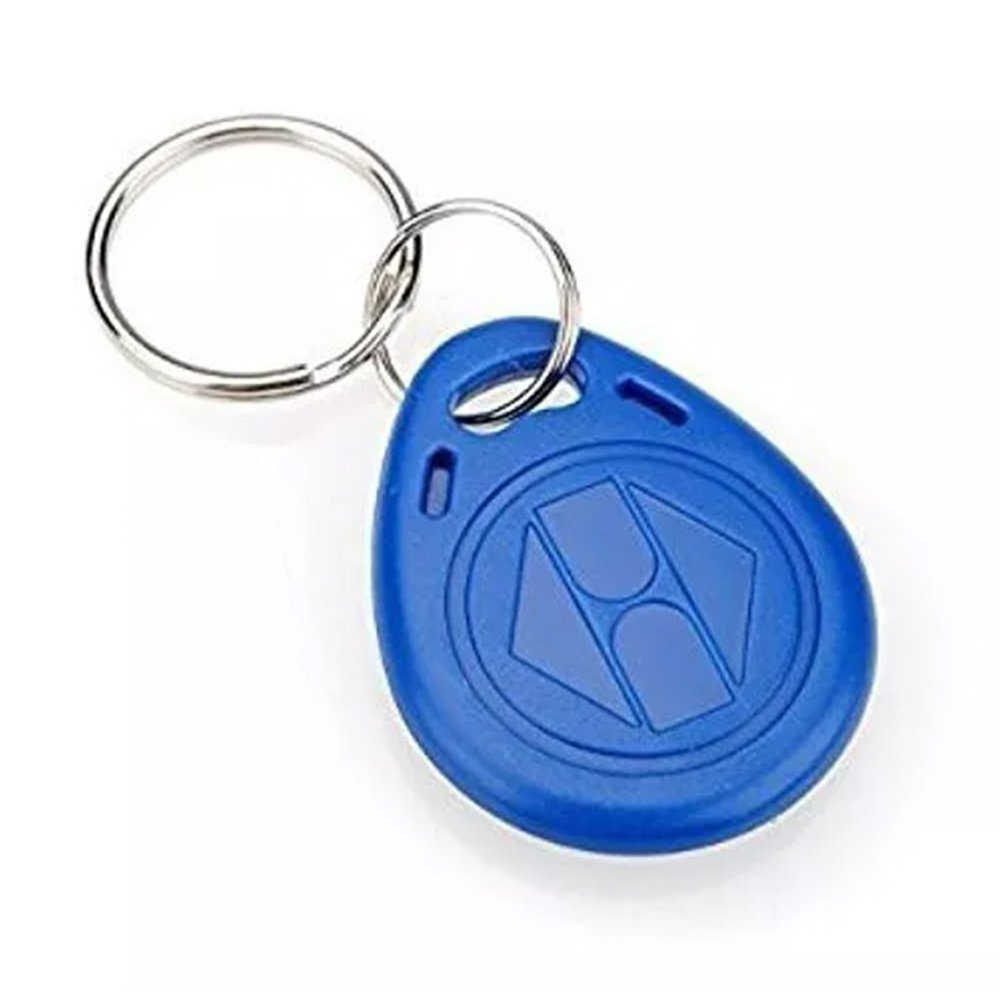
\includegraphics[width=0.7\textwidth]{llavero-rfid.jpg}
		\caption{Un llavero RFID}
	\end{subfigure}
	\begin{subfigure}{0.4\textwidth}
		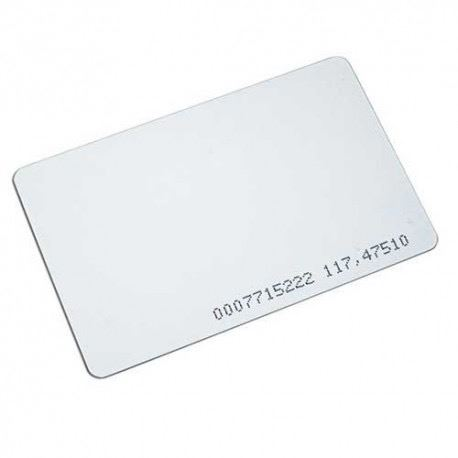
\includegraphics[width=0.7\textwidth]{tarjeta-rfid.jpg}
		\caption{Una tarjeta RFID}
	\end{subfigure}
	\caption{Distintos tags RFID}
\end{figure}

\clearpage
\subsubsection{Pinout del dispositivo}

\begin{wrapfigure}{r}{0in}
	\centering
	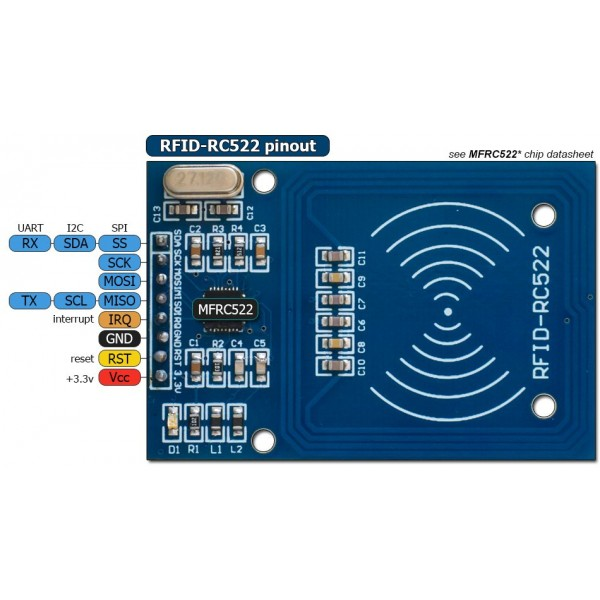
\includegraphics[width=0.5\textwidth]{rfid-rc522-pinout.jpg}
	\caption{El pinout del lector RFID-RC552.
		Se puede notar como este dispositivo está adaptado para funcionar con 3 protocolos
		distintos, comunicación por UART, comunicación por I2C y comunicacion por SPI}
\end{wrapfigure}

% la verdad es que este "---" esta RE mal, lo tendria que cambiar con titlesec

\paragraph{pin SDA ---}
Este pin se utiliza de forma distinta dependiendo del protocolo
de comunicación utilizado.
\begin{itemize}
	\item En I2C, se usa como el pin SDA.
	\item En UART, se usa como pin RX.
	\item En SPI, se usa como el pin SS
\end{itemize}

\paragraph{pin SCK ---}
El pin SCK se usa para mantener el sincronísmo con una señal de reloj

\paragraph{pin MOSI ---}
El pin MOSI sirve para hacer una transmisión Master Out - Slave In

\paragraph{pin MISO ---}
El pin MISO sirve para hacer una transmisión Master In - Slave Out

\paragraph{pin IRQ ---}
Se usa para las interrupciones

\paragraph{GND ---}
Sirve para mantener la referencia con Masa

\paragraph{RST ---}
Este pin sirve para resetear o desactivar el circuito integrado

\paragraph{VCC ---}
Pin de alimentación \textbf{3.3v}

\clearpage
\subsubsection{Mapeo de Memoria}
La identificación se realiza con unos llaveros o unas tarjetas,
que tienen este mapeo de memoria:

Tenemos 1k de memoria adentro de este chip, y la memoria EEPROM esta organizada de la
siguiente manera: Hay 16 sectores de 4 bloques, y cada bloque contiene 16 bytes.

\begin{figure}[H]
	\centering
	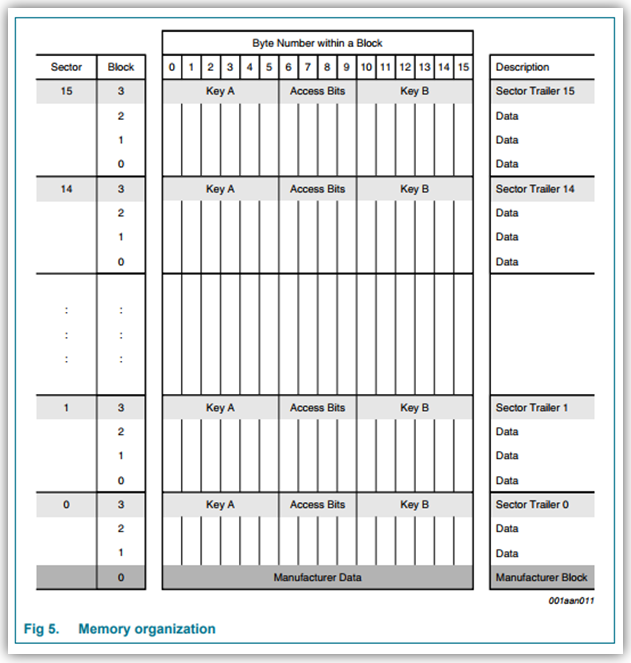
\includegraphics[width=0.7\textwidth]{rfid-mapeo-memoria.png}
\end{figure}

\end{document}